\documentclass[12pt,a4paper,faculty=ea,language=en,doctype=article]{ugent-doc}

% Optional: margins and spacing
%-------------------------------
% Uncomment and adjust to change the default values set by the template
% Note: the defaults are suggested values by Ghent University
\geometry{bottom=2.5cm,top=2.5cm,left=3cm,right=2cm} 
\renewcommand{\baselinestretch}{1.15}  %line spacing

% Font
%------
\usepackage[T1]{fontenc}
\usepackage[utf8]{inputenc} % allows non-ascii input characters
% Comment or remove the two lines below to use the default Computer Modern font
\usepackage{libertine}
\usepackage{libertinust1math}
% NOTE: because the UGent font Panno is proprietary, it is not possible to use it
% in Overleaf. But UGent does not suggest to use Panno for documents (or maybe only for
% the titlepage). For the body, the UGent suggestion is to use a good serif font (for
% LaTeX this could be libertine or Computer Modern).

% Proper word splitting
%-----------------------
\usepackage[english]{babel} 

% Mathematics
%-------------
\usepackage{amsmath}

% Figures
%---------
\usepackage{graphicx} % optional: the package is already loaded by the template
\graphicspath{{./figures/}}

% Bibliography settings
%-----------------------
\usepackage[backend=biber, style=apa, sorting=nyt, hyperref=true]{biblatex}
\addbibresource{./references.bib}
\usepackage{csquotes} % Suggested when using babel+biblatex

% Hyperreferences
%-----------------
\usepackage[colorlinks=true, allcolors=ugentblue]{hyperref}

% Whitespace between paragraphs and no indentation
%--------------------------------------------------
\usepackage[parfill]{parskip} 

% Input for title page
%----------------------

% The title
\thesubtitle{Linked Data LOL} % Optional

%% Note: a stricter UGent style could be achieved with, e.g.:
\usepackage{ulem} % for colored underline
\renewcommand{\ULthickness}{2pt} % adjust thickness of underline
\thetitle{\uline{\color{ugentblue} Augmented Reality visualisation on site:\newline BIM semantics and communication}}
% Note: do not forget to reset the \ULthickness to 1pt after invoking \maketitle
% (otherwise all underlines in the rest of your document will be too thick):
%\renewcommand{\ULthickness}{1pt}

% The first (top) infobox at bottom of titlepage
\infoboxa{\bfseries\large Master's dissertation submitted in order to obtain the academic degree of \newline
Master of Science in de ingenieurswetenschappen: architectuur
}

% The second infobox at bottom of titlepage
\infoboxb{Supervisors: 
\begin{tabular}[t]{lll}
    Prof.\ Dr.\ Paulus Present\\ % note syntax 'short space'
    Prof.\ Dr.\ Ruben Verstraeten\\
    Dr.\ Jeroen Werbrouck
\end{tabular}
}

% The third infobox at bottom of titlepage
\infoboxc{Philippe Soubrier 01702837 philippe.soubrier@ugent.be}

% The last (bottom) infobox at bottom of titlepage
\infoboxd{Academic year: 2022--2023} % note dash, not hyphen


\begin{document}

% =====================================================================
% Cover
% =====================================================================

% ------------ TITLE PAGE ---------
\maketitle
\renewcommand{\ULthickness}{1pt}

% =====================================================================
% Front matter
% =====================================================================

% ------------ TABLE OF CONTENTS ---------
{\hypersetup{hidelinks}\tableofcontents} % hide link color in toc
\newpage


% =====================================================================
% Main matter
% =====================================================================
\section*{Short summary}
\addcontentsline{toc}{section}{Short summary} % add unnumbered section to toc

This is a section without section number.
By default, unnumbered sections are ignored in the table of contents (toc).
Therefore an additional statement is necessary to make sure that this section is added to the toc.

The \verb|abstract| environment also works, but it does not look as nice (in my opinion) as an unnumbered section.

% ---------------------------------------------------------------------

\section{Introduction}

This example uses the article class as underlying document type, so there are no chapters.
Your introduction goes here! Simply start writing your document and use the Recompile button to view the updated PDF preview.
Examples of commonly used commands and features are listed below, to help you get started.

Once you're familiar with the editor, you can find various project setting in the Overleaf menu, accessed via the button in the very top left of the editor.
To view tutorials, user guides, and further documentation, please visit our \href{https://www.overleaf.com/learn}{help library}.

% ---------------------------------------------------------------------

\section{Some examples to get started}

\subsection{How to create Sections, Subsections and Subsubsections}

Simply use the section, subsection and subsubsection commands, as in this example document!
With Overleaf, all the formatting and numbering is handled automatically according to the template you've chosen.
If you're using Rich Text mode, you can also create new section and subsections via the buttons in the editor toolbar.

\subsubsection{Example subsubsection}

Here is an example of a subsubsection.
% ---------------------------------------------------------------------

\subsection{How to include Figures}

First you have to upload the image file from your computer using the upload link in the file-tree menu.
In the preamble the location where the images/figures are located was defined, i.e. \verb|\graphicspath{{./figures/}}|.
So, put your images/figures in that folder.
Then use the includegraphics command to include it in your document.
Use the figure environment and the caption command to add a number and a caption to your figure.
See the code for Figure \ref{fig:frog} in this subsection for an example.

\begin{figure}[ht]
	\centering
	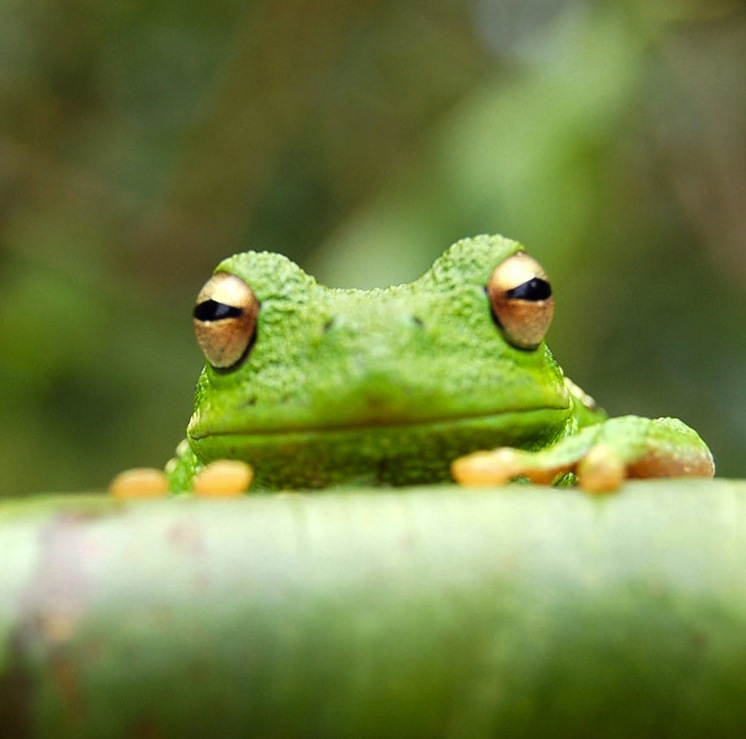
\includegraphics[width=0.3\textwidth]{frog.jpg}
	\caption{\label{fig:frog}This is an example image.}
\end{figure}

Note that your figure will automatically be placed in the most appropriate place for it, given the surrounding text and taking into account other figures or tables that may be close by.
You can find out more about adding images to your documents in this help article on \href{https://www.overleaf.com/learn/how-to/Including_images_on_Overleaf}{including images on Overleaf}.

% ---------------------------------------------------------------------

\subsection{How to add Tables}

Use the table and tabular environments for basic tables --- see Table~\ref{tab:widgets}, for example.
For more information, please see this help article on \href{https://www.overleaf.com/learn/latex/tables}{tables}.

\begin{table}[h]
	\centering
	\begin{tabular}{l|r}
		Item    & Quantity \\\hline
		Widgets & 42       \\
		Gadgets & 13
	\end{tabular}
	\caption{\label{tab:widgets}An example table.}
\end{table}

% ---------------------------------------------------------------------

\subsection{How to add Lists}

You can make lists with automatic numbering \dots

\begin{enumerate}
	\item Like this,
	\item and like this.
\end{enumerate}
\dots or bullet points \dots
\begin{itemize}
	\item Like this,
	\item and like this.
\end{itemize}
\dots or custom lists \dots
\begin{itemize}
	\item[a.] Like this,
	\item[b.] and like this.
\end{itemize}

Note that specialized packages exist that give you more flexible ways of creating lists (for example \verb|enumitem|).

% ---------------------------------------------------------------------

\subsection{How to write Mathematics}

\LaTeX{} is great at typesetting mathematics.
Let $X_1, X_2, \ldots, X_n$ be a sequence of independent and identically distributed random variables with $\text{E}[X_i] = \mu$ and $\text{Var}[X_i] = \sigma^2 < \infty$, and let
\[S_n = \frac{X_1 + X_2 + \cdots + X_n}{n}
	= \frac{1}{n}\sum_{i}^{n} X_i\]
denote their mean.
Then as $n$ approaches infinity, the random variables $\sqrt{n}(S_n - \mu)$ converge in distribution to a normal $\mathcal{N}(0, \sigma^2)$.

% ---------------------------------------------------------------------

\subsection{How to change the spell check settings}

To change the spell check language, simply open the Overleaf menu at the top left of the editor window, scroll down to the spell check setting, and adjust accordingly.

% ---------------------------------------------------------------------

\subsection{How to add Citations and a References List}

You can simply upload a \texttt{.bib} file containing your BibTeX entries, created with a tool such as JabRef.
Alternatively, you can manually appendix BibTex entries to the \texttt{references.bib} file available on e.g. Google Scholar. You can then cite entries from it, like this: \textcite{greenwade93} or \parencite{greenwade93}.

% ---------------------------------------------------------------------

\subsection{Good luck!}

We hope you find Overleaf useful, and do take a look at our \href{https://www.overleaf.com/learn}{help library} for more tutorials and user guides! Please also let us know if you have any feedback using the Contact Us link at the bottom of the Overleaf menu --- or use the contact form at \url{https://www.overleaf.com/contact}.


% =====================================================================
% End matter
% =====================================================================

% ------------ REFERENCES ------------
\printbibliography[heading=bibintoc,title={References}] % check if bibliography is in table of contents


% ------------ APPENDIX ------------
\appendix
\section{Appendix: Your first appendix}
Insert some figure or table here.

\newpage
\section{Appendix: Your second appendix}
The second appendix was forced to start on a new page.

\end{document}
